Uživatelská funkce je funkce, která nezná vnitřní implementaci tnumů (jako funkcí přesnosti) a volá jen funkce rozhraní zobrazené v Tabulce \ref{tab:funkce_rozhrani}. Během programování knihovny již některé mimoděk vznikly (například \texttt{tnum-}), v této kapitole nějaké přidáme. Ukážeme, že síla knihovny spočívá v jednoduchém vytváření nových tnumů a ve velmi silně oddělené vnitřní implementaci od vnějšího chování.

\subsection{Instalace}\label{ssec:inst}
Knihovna \texttt{tnums} je k dostání na githubu na odkaze \url{https://github.com/slavon00/tnums} nebo pro čtenáře tištěné verze na přiloženém fyzickém disku. Je to Lispová knihovna, od uživatele se předpokládá znalost základů práce s Lispem.

Vše, co jsme doposud naprogramovali najdeme v souboru \texttt{src/tnums.lisp} a všechny funkce, které přidáme v této kapitole, pak v \texttt{src/user-functions.lisp}. Testy, které budu ukazovat jsou v souboru \texttt{src/tests.lisp}. Vše je možné jednoduše načíst evaluací souboru \texttt{load.lisp}, jak ukazuje Obrázek \ref{obr:loading}. Pro kompletní obsah adresáře vizte přílohu \ref{pril:adresar}.

Knihovna se v budoucnosti může měnit, takže tyto informace mohou zastarat. Knihovna na githubu bude ale vždy obsahovat soubor \texttt{README.md} nebo ekvivalentní, s popisem postupu instalace.

\begin{myfigure}{H}
\caption{Načtení knihovny \texttt{tnums} do \texttt{SBCL}}
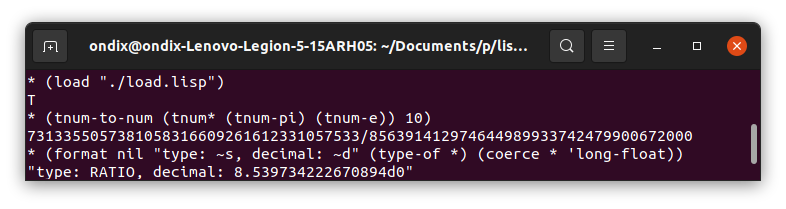
\includegraphics[width=\linewidth]{./graphics/loading2.png}\label{obr:loading}
Aby se nemusely ručně načítat všechny soubory, lze knihovnu \texttt{tnums} též načíst jen evaluací souboru \texttt{load.lisp}. 
\end{myfigure}

\subsection{Převody a konstanty}
Téměř všechny naprogramované funkce berou jako vstup tnumy. To jsou abstraktní struktury (vyjadřující rekurzivní čísla), které interně reprezentujeme jako funkce malých čísel. K vytvoření tnumu z čísla slouží funkce \texttt{num-to-tnum}.

\begin{lisptest}{\texttt{num-to-tnum}}{Představení funkce pro převod $\mathbb{R}\to\mathfrak{T}$}
* (num-to-tnum 42.123)
#<FUNCTION (LAMBDA (EPS) :IN NUM-TO-TNUM) {10020A056B}>
\end{lisptest}

Pro převod opačným směrem slouží inverzní funkce \texttt{tnum-to-num}, která bere tnum a druhý argument představující přesnost, se kterou chceme tnum vyčíslit.

\begin{lisptest}{\texttt{tnum-to-num}}{Představení funkce pro převod $\mathfrak{T}\to\mathbb{Q}$}
* (tnum-to-num * 0.1)
34246/813
\end{lisptest}

Výsledkem vyčíslení je racionální číslo.

\begin{lisptest}{Typ výstupu je číslo}{Ověření typu vraceného numu}
* (type-of *)
RATIO
* (float **)
42.123
\end{lisptest}

Výsledkem vyhodnocení je číslo, které můžeme použít jako vstup do dalších funkcí. Naprogramujme nyní funkci, která bude tnumy převádět na textové řetězce. Takto získáme dlouhé rozvoje v čitelné podobě namísto velkých zlomků.

\begin{lispcode}{\texttt{tnum-to-string}}{Funkce na převod tnumu na textový řetězec}
(\textcolor{funkcionalni}{defun} \textcolor{pojmenovan}{tnum-to-string} (tnum count)
  (\textcolor{vedlejsi}{let} ((num (\textcolor{moje}{tnum-to-num} tnum (\textcolor{matematicke}{1+} count))) (output ""))
    (\textcolor{vedlejsi}{flet} ((get-digit (&optional (end ""))
             (\textcolor{matematicke}{multiple-value-bind} (digit rem) (\textcolor{matematicke}{floor} num)
               (\textcolor{vedlejsi}{setf} output (\textcolor{matematicke}{concatenate} \textquotesingle\textcolor{moje}{string} output 
                                         (\textcolor{funkcionalni}{write-to-string} digit)
                                         end)
                     num (\textcolor{matematicke}{*} 10 rem)))))
      (\textcolor{funkcionalni}{when} (\textcolor{matematicke}{<} num 0) (\textcolor{vedlejsi}{setf} output "-" num (\textcolor{matematicke}{-} num)))
      (\textcolor{moje}{get-digit} ".")  
      (\textcolor{funkcionalni}{dotimes} (i count (\textcolor{matematicke}{concatenate} \textquotesingle\textcolor{moje}{string} output "..."))
        (\textcolor{moje}{get-digit})))))
\end{lispcode}
Funkce bere jako vstup tnum a přirozené číslo značící počet desetinných míst, která má řetězec obsahovat. Otestujeme ji na výpisu Ludolfova čísla.

\begin{lisptest}{\texttt{tnum-string} a \texttt{tnum-pi}}{Vyčíslení Ludolfova čísla na přesnost 50 desetinných míst}
* (tnum-to-string (tnum-pi) 50)
"3.14159265358979323846264338327950288419716939937510..."
\end{lisptest}

Vzhledem k rozšíření množiny přípustných hodnot druhého parametru funkce \texttt{tnum-to-num} mimo $(0,1)$ je možné pohodlně přepínat mezi návratovou hodnotou jako číslem a textovým řetězcem. Ukážeme si to na vyčíslení Eulerova čísla.

\begin{lisptest}{\texttt{tnum-string} a \texttt{tnum-e}}{Vyčíslení Eulerova čísla na přesnost 20 desetinných míst a jeho vrácení jako čísla a jako stringu}
* (tnum-to-num (tnum-e) 20)
611070150698522592097/224800145555521536000
* (tnum-to-string (tnum-e) 20)
"2.71828182845904523536..."
\end{lisptest}

\subsection{Operace}
Operace tnumu je funkce $\bigtimes_{i=0}^{n-1}\mathfrak{T}\rightarrow\mathfrak{T}$, kde $n\in\mathbb{N}$ nazýváme aritou. Operace \texttt{tnum+} a \texttt{tnum*} mohou mít libovolný počet argumentů, operace \texttt{-tnum} a \texttt{/tnum} jsou striktně unární, operace \texttt{tnum-} a \texttt{tnum/} potřebují alespoň jeden argument a operace \texttt{tnum-expt} a \texttt{tnum-root} jsou binární.

V lispu jsou dvě šikovné funkce na inkrementaci a dekrementaci čísla. To samé nyní přidáme pro tnumy.

\begin{lispcode}{\texttt{tnum-1+}}{Funkce pro inkrementaci tnumu o jedničku}
(\textcolor{funkcionalni}{defun} \textcolor{pojmenovan}{tnum-1+} (tnum)
  (\textcolor{moje}{tnum+} (\textcolor{moje}{num-to-tnum} 1) tnum))
\end{lispcode}

Funkce pro dekrementaci se také dá napsat pohodlně uživatelsky.

\begin{lispcode}{\texttt{tnum-1-}}{Funkce pro dekrementaci tnumu o jedničku}
(\textcolor{funkcionalni}{defun} \textcolor{pojmenovan}{tnum-1-} (tnum)
  (\textcolor{moje}{tnum-} tnum (\textcolor{moje}{num-to-tnum} 1)))
\end{lispcode}

Také by šla napsat nejpoužívanější odmocnina a sice druhá.

\begin{lispcode}{\texttt{tnum-sqrt}}{Funkce pro druhou odmocninu tnumu}
(\textcolor{funkcionalni}{defun} \textcolor{pojmenovan}{tnum-sqrt} (tnum)
  (\textcolor{moje}{tnum-root} (\textcolor{moje}{num-to-tnum} 2) tnum))
\end{lispcode}

Výše naprogramované použijeme k zavedení další konstanty, zlatého řezu.

\begin{definition}[Zlatý řez \cite{GR}]
Zlatý řez představuje kladné řešení rovnice \\$x^2-x-1=0$, je tedy roven hodnotě
\begin{equation}
\varphi=\frac{1+\sqrt{5}}{2}.
\end{equation}
\end{definition}

Jedná se o další iracionální konstantu, tentokrát algebraickou, protože je řešením algebraické rovnice a její tnum je jen syntaktický přepis uvedené definice.

\begin{lispcode}{\texttt{tnum-phi}}{Funkce pro tnum Zlatého řezu}
(\textcolor{funkcionalni}{defun} \textcolor{pojmenovan}{tnum-phi} ()
  (\textcolor{moje}{tnum/} (\textcolor{moje}{tnum-1+} (\textcolor{moje}{tnum-sqrt} (\textcolor{moje}{num-to-tnum} 5))) (\textcolor{moje}{num-to-tnum} 2)))
\end{lispcode}

A ještě test.

\begin{lisptest}{\texttt{tnum-phi}}{Představení funkce pro zlatý řez}
* (tnum-to-string (tnum-phi) 50)
"1.61803398874989484820458683436563811772030917980576..."
\end{lisptest}

\subsection{Funkce}
Funkce tnumů jsou všechny unární. Jedná se o přirozený logaritmus, goniometrické funkce a exponenciálu. Omezení definičního oboru jsou stejná jako jsme zvyklí, naprogramované funkce tedy nejsou o nic \uv{slabší}.

Exponenciálu jsme využili už při psaní obecné mocniny. V podobném duchu nyní zavedeme obecný logaritmus. Vyjdeme z faktu, že lze převádět mezi různými základy.

\begin{fact}[Obecný logaritmus jako podíl přirozených  \cite{tabulky}]
Pro $a>1$ a $x\in\mathbb{R}^+$ platí
\begin{equation}
\log_a(x)=\frac{ln(x)}{ln(a)}
\end{equation}
\end{fact}

Nová funkce bude brát dva argumenty, a proto nejde tak úplně o funkci tnumu jak ji v této práci chápeme, ale spíše o matematickou operaci. Nicméně na eleganci zápisu to nic neubírá.

\begin{lispcode}{\texttt{tnum-log}}{Funkce pro výpočet obecného logaritmu}
(\textcolor{funkcionalni}{defun} \textcolor{pojmenovan}{tnum-log} (tnum1 tnum2)
  (\textcolor{moje}{tnum/} (\textcolor{moje}{tnum-ln} tnum2) (\textcolor{moje}{tnum-ln} tnum1)))
\end{lispcode}

Uživatelská funkce potom podobně jako u odmocniny prohazuje argumenty, protože mluvíme vždy o nějakém logaritmu něčeho, například \uv{devítkový logaritmus dvou}. Ten je i předmětem následujícího testu.

\begin{lisptest}{\texttt{tnum-log}}{Vyčíslení devítkového logaritmu dvou}
* (tnum-to-string (tnum-log (num-to-tnum 9) (num-to-tnum 2)) 50)
"0.31546487678572871854976355717138042714979282006594..."
\end{lisptest}

Goniometrické funkce jsou z velké části napsány též uživatelsky, takže by mělo být jasné, jak se s nimi z tohoto pohledu pracuje. Ukážu tedy jen vyčíslení, aby bylo vidět, že funkce opravdu fungují. Následuje výpočet sinu jedničky.

\begin{lisptest}{\texttt{tnum-sin}}{Představení funkce na výpočet sinu tnumu}
* (coerce (tnum-to-num (tnum-sin (num-to-tnum 1)) -20)
    'long-float)
0.8414709848078965d0
\end{lisptest}

\subsection{Rychlost}
Tabulka \ref{tab:rychlost} zobrazuje, jak dlouho běžně trvá vyhodnocení výrazů. Konkrétní hodnoty budou vždy závislé na konkrétním stroji a jeho momentálním zatížení, obecnou představu o časové náročnosti výpočtů však poskytují.

\begin{table}[H]
\begin{mdframed}[backgroundcolor=lightpink,innertopmargin=-2.5pt,innerbottommargin=2.5pt]
\centering
\caption{Doba výpočtů daných výrazů}
\label{tab:rychlost}
\begin{tabular}{| >{\columncolor[gray]{1}} l |>{\columncolor[gray]{1}}p{2.5cm}|}
\hline
\multicolumn{1}{|>{\columncolor[gray]{1}}c|}{Výraz} & Doba vyhodnocení~(s)\\\hline\hline
\texttt{((let ((tn}& \cellcolor[gray]{1} \\
\texttt{~~~~~~(tnum/ (tnum-pi) (tnum-e) (tnum-phi)))} & \multirow{-2}{*}{-}\\ \hline
\texttt{~~~(tnum-to-string tn 50)} & 0.427424 \\ \hline
\texttt{~~~(tnum-to-string (tnum-sin tn) 50)} & 31.412191 \\ \hline
\texttt{~~~(tnum-to-string (tnum-csc tn) 50)} & 4690.939552 \\ \hline
\texttt{~~~(tnum-to-string (tnum-ctan tn) 50))} & 26756.683374 \\ \hline
\end{tabular}

Tabulka v prvním sloupci zobrazuje výrazy, které byly vyhodnocovány, a ve druhém čas, který toto vyhodnocení zabralo. Doba byla měřena makrem \texttt{time} a hodnoty jsou z řádku \uv{(\ldots) seconds of total run time}.
\end{mdframed}
\end{table}

\subsection{Vnější volání}
Rozhraní knihovny \texttt{tnums} -- funkce určené k volání uživatelem -- zobrazuje Tabulka \ref{tab:funkce_rozhrani}.

\begin{table}[H]
\begin{mdframed}[backgroundcolor=lightpink,innertopmargin=-2.5pt,innerbottommargin=2.5pt]
\centering
\caption{Funkce nabízené knihovnou \texttt{tnums}}
\label{tab:funkce_rozhrani}
\begin{tabular}{| >{\columncolor[gray]{1}} c |>{\columncolor[gray]{1}}c|>{\columncolor[gray]{1}}p{4.8cm}|}
\hline
Název & Argumenty & Význam\\ \hline \hline
\texttt{tnum-to-num} & \texttt{tnum:tnum}, \texttt{eps:num} & převod \texttt{tnum}u na číslo s~přesností \texttt{eps}\\
\texttt{tnum-to-string} & \texttt{tnum:tnum}, \texttt{count:num} & převod \texttt{tnum}u na textový řetězec o \texttt{count} desetinných místech\\\hline
\texttt{num-to-tnum}&\texttt{num:num}&převod \texttt{num}u na tnum\\
\texttt{tnum-pi}&$\emptyset$&tnum Ludolfova čísla\\
\texttt{tnum-e}&$\emptyset$&tnum Eulerova čísla\\
\texttt{tnum-phi}&$\emptyset$&tnum Zlatého řezu\\\hline
\texttt{-tnum}&\texttt{tnum:tnum}&$-\texttt{tnum}$\\
\texttt{tnum+}&0+ \texttt{tnum}ů&tnumovský protějšek \texttt{+}\\
\texttt{tnum-}&1+ \texttt{tnum}ů&numovský protějšek \texttt{-}\\
\texttt{/tnum}&\texttt{tnum:tnum}&$1/\texttt{tnum}$\\
\texttt{tnum*}&0+ \texttt{tnum}ů&numovský protějšek \texttt{*}\\
\texttt{tnum/}&1+ \texttt{tnum}ů&numovský protějšek \texttt{/}\\
\texttt{tnum-expt}&\texttt{arg1:tnum}, \texttt{arg2:tnum}&$\texttt{arg1}^{\texttt{arg2}}$\\
\texttt{tnum-sqrt}&\texttt{arg1:tnum}, \texttt{arg2:tnum}&$\sqrt[\texttt{arg1}]{\texttt{arg2}}$\\
\texttt{tnum-log}&\texttt{arg1:tnum}, \texttt{arg2:tnum}&$\mathrm{log}_{\texttt{arg1}}(\texttt{arg2})$\\
\texttt{tnum-1+}&\texttt{tnum:tnum}&$\texttt{tnum} + 1$\\
\texttt{tnum-1-}&\texttt{tnum:tnum}&$\texttt{tnum} - 1$\\\hline
\texttt{tnum-exp}&\texttt{tnum:tnum}&přirozená mnocnina \texttt{tnum}u\\
\texttt{tnum-ln}&\texttt{tnum:tnum}&přirozený logaritmus \texttt{tnum}u\\
\texttt{tnum-sqrt}&\texttt{tnum:tnum}&druhá odmocnina \texttt{tnum}u\\
\texttt{tnum-sin}&\texttt{tnum:tnum}&sinus \texttt{tnum}u\\
\texttt{tnum-cos}&\texttt{tnum:tnum}&kosinus \texttt{tnum}u\\
\texttt{tnum-tan}&\texttt{tnum:tnum}&tangens \texttt{tnum}u\\
\texttt{tnum-csc}&\texttt{tnum:tnum}&kotangens \texttt{tnum}u\\
\texttt{tnum-sec}&\texttt{tnum:tnum}&sekans \texttt{tnum}u\\
\texttt{tnum-ctan}&\texttt{tnum:tnum}&kosekans \texttt{tnum}u\\
\hline\end{tabular}

Tabulka v prvním sloupci zobrazuje funkční symbol, v posledním význam funkce aplikované na argumenty z prostředního sloupce. Čtyři části rozdělené horizontálními čarami jsou po řadě funkce pro převody, konstanty, operace a matematické funkce. Součástí jsou i uživatelské funkce.
\end{mdframed}
\end{table}